\pattern{Distributed}
\begin{summary}
Distributed objects is a combination and adaptation of many simpler
architectures. It is derived from object-oriented and client-server
architecture which allows for objects to be distributed and accessed. When
developing applications using this architecture, it is very easy to come across
some constraints such as cross-machine and cross-language communication. To
address this, additional styles are applied such as pipe-filtering which allow
for serialization of parameters which creates uniform communication. This
process of filtering, serializing parameters is known as data marshaling.
\end{summary}

\comparison{\begin{itemize}
        \item Engender change resilience: The increased redundancy in a
            distributed system can increase its resiliency. Hardware is prone
            to failure, so by distributing the functionality and data across a
            cluster of machines, this allows the system to recover from
            unforeseen crashes. When certain machines are down, the system can
            still retain its full functionality since the remaining nodes in
            the cluster are able to pick up the slack by doing its work. For
            this to work, the data is also stored redundantly amongst the
            cluster to ensure that a copy of the data is always available even
            when a portion of the cluster is offline. By the nature of its
            design, distributed objects also makes the system more scalable.
            When there is a big increase in demand, the cluster manager can
            spin up more machines in the cluster during runtime to accommodate
            for the extra requests. The performance and resiliency of a cluster
            can be changed without altering its functionality, this is done by
            changing the size of the cluster.
\end{itemize}
}{\begin{itemize}
        \item Using distributed objects allows systems to be designed and
            developed using segments that are written in different languages
            with different platforms. However, this induces the applications to
            be built in the distributed objects style. The first negative
            behaviour is exhibited in the interactions of components, it tends
            to be mostly synchronous and it does not take the advantage of
            distributed systems concurrency. In terms of object interactions,
            many distributed object style applications may have trouble dealing
            with data traversal in streams, and also having difficulties with
            asynchronous invocations. This induces the distributed objects
            style on the application building process without regarding if it’s
            the best style for the application.

        \item In terms of the components in a distributed objects style,
            they are required to explicitly specify the provided interfaces,
            however, it does not specifying required interfaces, which may
            cause deeply ingrained dependencies between objects. Another
            negative behaviour exhibiting from distributed objects style is
            that the objects are created, linked, and destroyed constantly. Due
            to all the creation and destruction of the objects, it’s difficult
            to fully comprehend the structure and configurations of the
            application at any given time.
\end{itemize}}

\begin{nfps}
\item[None] Gonna have to dig in the rest of this text for them.
\end{nfps}

\subsubsection{Implementation}

Implementation of Distributed Objects may involve several important
aspects. Firstly, a class named “Matrix Class” is initialized in a generic,
broad object language. That matrix class actually defines the inner components
and functions like methods. Most of the times, such is IDL: Interface
Description Language.
At the very initial stage of compilation, the matrix class is changed to every
listed languages, whether they be C++, Java, etc. Every program subsequently
involves the feasible file in their system. These blocks of codes comprise of
the definition of classes as well as methods for disintegrating the actual
class to several components. This transmits them via a connection to other
program, regenerating the object on the opposite side.

\begin{center}
    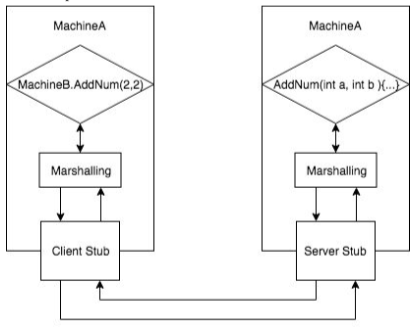
\includegraphics[width=0.48\textwidth]{./distributed1}
    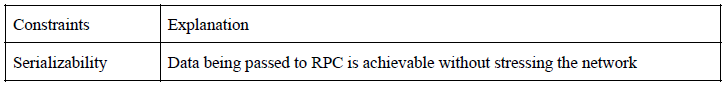
\includegraphics[width=0.48\textwidth]{./distributed2}
    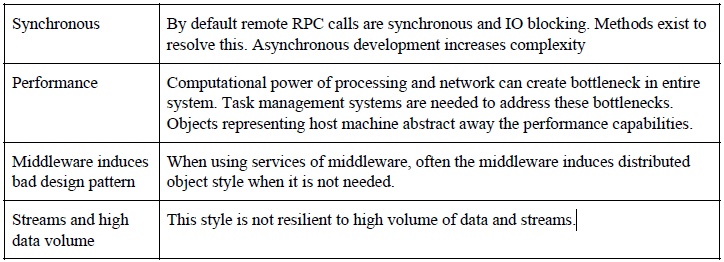
\includegraphics[width=0.48\textwidth]{./distributed3}
    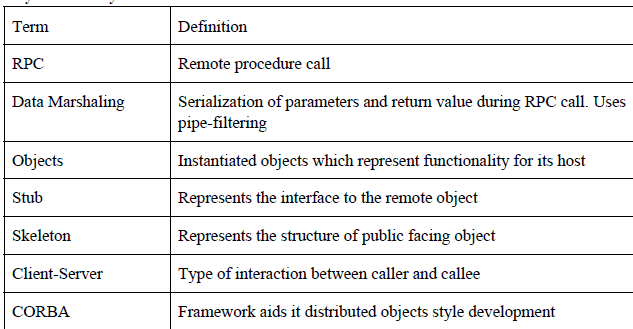
\includegraphics[width=0.48\textwidth]{./distributed4}
\end{center}
